\section{Polymorphie}


\begin{frame}
	\frametitle{Polymorphie}
	\begin{itemize}
		\item Gleiches Interface für Objekte von verschiedenen Typen
		\item Gegenteil: Monomorphie
	\end{itemize}
	\begin{table}[h]
	\begin{tabularx}{\textwidth}{$l|^X|^X}
		\rowstyle{\bfseries}  & universell                              & ad-hoc                             \\
		\rowstyle{\small}     & unendlich viele Typen                   & endliche Anzahl an Typen           \\
		\rowstyle{\small}     & eine Implementierung                    & unterschiedliche Implementierungen \\
		\hline
		\bfseries dynamisch   & \multirow{2}{*}{Inklusionspolymorphie/} &                                    \\
		\small    Laufzeit    & \multirow{2}{*}{Vererbungspolymorphie}  &                                    \\
		\small    langsamer   &                                         &                                    \\
		\hline
		\bfseries statisch    & \multirow{2}{*}{parametrische}          & \multirow{2}{*}{Überladung,}        \\
		\small    Kompilezeit & \multirow{2}{*}{Polymorphie}            & \multirow{2}{*}{Coercion}          \\
		\small    schneller   &                                         &                                    \\
	\end{tabularx}
\end{table}

	\begin{itemize}
		\item Statisch: es steht zur Kompilezeit fest, welche Funktion aufgerufen wird
		\item Dynamisch: es wird erst zur Laufzeit bestimmt, welche Funktion aufgerufen wird
	\end{itemize}
\end{frame}


\begin{frame}
	\frametitle{universelle Polymorphie}
	\begin{itemize}
		\item Gleiches Interface für unendlich viele Typen
		\item Eine Implementierung
		\item ``echte Vielgestaltigkeit''
		\item Inklusionspolymorphie
		\item Vererbungspolymorphie
		\item Parametrische Polymorphie
	\end{itemize}
\end{frame}


\begin{frame}
	\frametitle{Inklusionspolymorphie}
	\begin{itemize}
		\item Liskovsches Substitutionsprinzip ist erfüllt
		\begin{itemize}
			\item Objekt des Typen A kann problemlos, durch Objekt des Typen B ersetzt werden 
		\end{itemize}
	\end{itemize}
\end{frame}


\begin{frame}
	\frametitle{Vererbungspolymorphie}
	\begin{itemize}
		\item Dynamisch
		\item Kann Inklusionspolymorphie ausdrücken
		\item Sollte auch das Liskovsche Substitutionsprinzip befolgen, muss aber nicht
		\item Virtuelle Methoden
	\end{itemize}
\end{frame}


\begin{frame}
	\frametitle{Beispiel1: Fahrzeug (Vererbungspolymorphie)}
	{\tiny\UseRawInputEncoding{\lstinputlisting[language={C++}]{polymorphie/universell/vererbung/beispiele/fahrzeug/fahrzeug.good.cpp}}\inputencoding{utf8}}
\end{frame}


\begin{frame}
	\frametitle{Beispiel1: Fahrzeug (Mehrfache Auswahl)}
	{\tiny\UseRawInputEncoding{\lstinputlisting[language={C++}]{polymorphie/universell/vererbung/beispiele/fahrzeug/fahrzeug.bad.cpp}}\inputencoding{utf8}}
\end{frame}


\begin{frame}
	\frametitle{Beispiel2: Snake}
	\begin{figure}[H]
		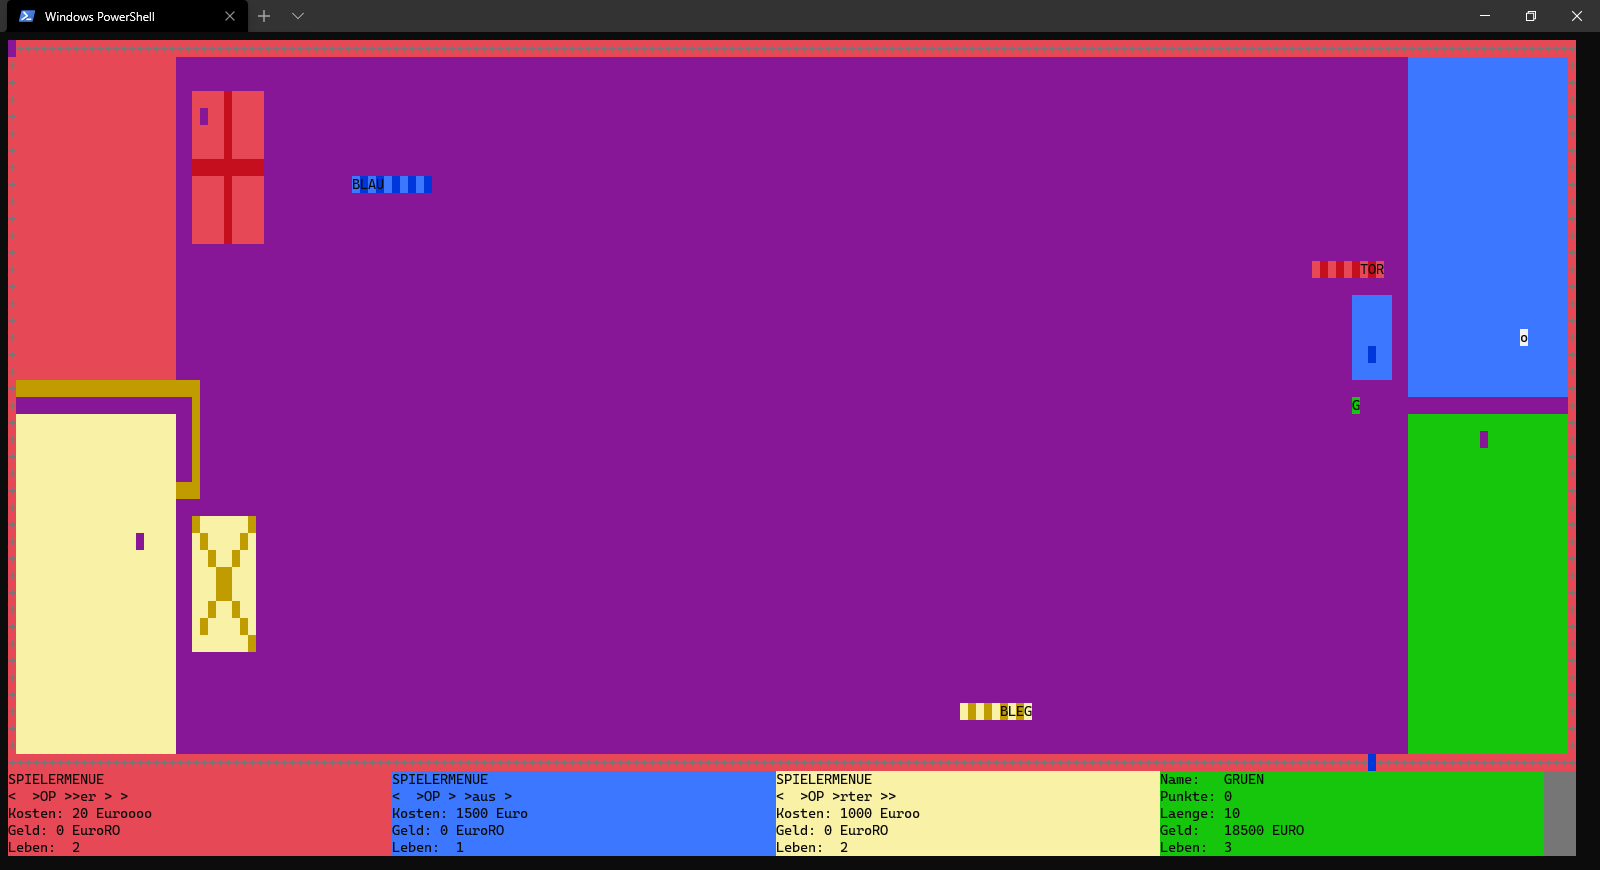
\includegraphics[width=\textwidth]{polymorphie/universell/vererbung/beispiele/snake/snake.png}
	\end{figure}
\end{frame}


\begin{frame}
	\frametitle{Beispiel2: Snake}
	\begin{itemize}
		\item Unterschiedliche Arten von Gebäuden (Kanonen, Mauern, Geldlager, Krankenhäuser, ...)
		\item Unterschiedliche Arten von Punkten (normale Punkte, Geld, Leben, ...)
	\end{itemize}
\end{frame}


\begin{frame}
	\frametitle{Beispiel2: Mein Code (nicht nachmachen!)}
	{\tiny\UseRawInputEncoding{\lstinputlisting[language={C++}]{polymorphie/universell/vererbung/beispiele/snake/snake_gebaeude.bad.cpp}}\inputencoding{utf8}}
\end{frame}

\begin{frame}
	\frametitle{Beispiel2: Mit Vererbungspolymorphie}
	\begin{figure}[H]
		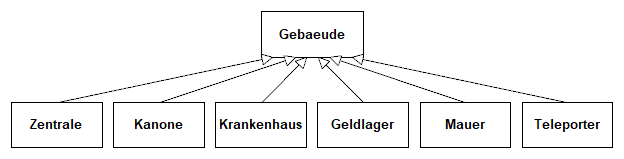
\includegraphics[width=\textwidth]{polymorphie/universell/vererbung/beispiele/snake/gebaeude.png}
	\end{figure}
	{\tiny\UseRawInputEncoding{\lstinputlisting[language={C++}]{polymorphie/universell/vererbung/beispiele/snake/snake_gebaeude.good.cpp}}\inputencoding{utf8}}
\end{frame}

\begin{frame}
	\frametitle{Kreis-Ellipse-Problem}
	\begin{itemize}
		\item Problem:
		\begin{itemize}
			\item Basisklasse 'Form' hat die Methoden 'zeichnen' und 'flaeche'
			\item Ellipsen und Kreise sollen erstellt werden können
			\item 'Kreis' erbt von 'Ellipse' erbt von 'Form'
			\item Bei Kreisen können nicht beide Dimensionen unabhängig voneinander skaliert werden
			\item Liskovsches Substitutionsprinzip nicht erfüllt
		\end{itemize}
		
		\item Lösungsvorschläge:
		\begin{itemize}
			\item Fehler bei Größenänderung
			\item Ellipse erbt von Kreis ab
			\item Keine Klasse Kreis
			\item Keine Vererbungsbeziehung zwischen Ellipse und Kreis
			\item Einführen neuer Basisklasse
		\end{itemize}
		
		\item Keiner der Lösungsvorschläge ist ideal
		\item Nicht jede ``ist-ein''-Beziehung sollte durch öffentliche Vererbung dargestellt werden!
	\end{itemize}
\end{frame}


\begin{frame}
	\frametitle{Parametrische Polymorphie (TODO)}
	\begin{itemize}
		\item Statisch
	\end{itemize}
\end{frame}


\begin{frame}
	\frametitle{Ad-hoc-Polymorphie}
	\begin{itemize}
		\item Gleiche Schnittstelle für begrenzte Anzahl an bestimmten Typen
		\item Eine Implementierung pro Typ
		\item Coercion
		\item Überladung
	\end{itemize}
\end{frame}


\begin{frame}
	\frametitle{Coercion}
	\begin{itemize}
		\item Statisch
		\item Implizite Typumwandlung
	\end{itemize}
	{\tiny\UseRawInputEncoding{\lstinputlisting[language={C++}]{polymorphie/adhoc/coercion/beispiele/src/eingebauteDatentypen.cpp}}\inputencoding{utf8}}
\end{frame}

\begin{frame}
	\frametitle{Coercion - Konvertierungskonstruktor}
	{\tiny\UseRawInputEncoding{\lstinputlisting[language={C++}]{polymorphie/adhoc/coercion/beispiele/src/konvertierungskonstruktoren.cpp}}\inputencoding{utf8}}
\end{frame}

\begin{frame}
	\frametitle{Coercion - Konvertierungsoperator}
	{\tiny\UseRawInputEncoding{\lstinputlisting[language={C++}]{polymorphie/adhoc/coercion/beispiele/src/konvertierungsoperatoren.cpp}}\inputencoding{utf8}}
\end{frame}


\begin{frame}
	\frametitle{Überladung}
	\begin{itemize}
		\item Statisch
		\item Mehrere Funktionen haben den gleichen Namen
		\item Operatorüberladung
	\end{itemize}
	{\tiny\UseRawInputEncoding{\lstinputlisting[language={C++}]{polymorphie/adhoc/ueberladung/beispiele/src/reset.cpp}}\inputencoding{utf8}}
\end{frame}
